\documentclass[tikz,border=10pt]{standalone}
\usetikzlibrary{shapes.geometric, arrows}


%defineixo el groc fosforito i blau cian
\definecolor{yellowfosforito}{RGB}{255,255,0}
\definecolor{blauCian}{RGB}{0, 255, 255}
\definecolor{taronjaBrillant}{RGB}{255, 140, 0}

% Estilos de los nodos y flechas
\tikzstyle{trapeziSortida} = [rectangle, minimum width=4.5cm, minimum height=1cm, text centered, draw=black, fill=taronjaBrillant!90]

%ELS TRAPEZIS QUEDEN MALAMENT I S'HAN SUBSTITUITS PER RECTANGLES
%\tikzstyle{trapeziSortida} = [trapezium, trapezium left angle=75, trapezium right angle=105, minimum height=.75cm, text centered, draw=black, fill=taronjaBrillant!90, font=\normalsize]


\tikzstyle{decisionBackend} = [diamond, minimum width=3cm, minimum height=1cm, text centered, draw=black, fill=yellowfosforito]
\tikzstyle{decisionFrontend} = [diamond, minimum width=3cm, minimum height=2cm, text centered, draw=black, fill=blauCian]
\tikzstyle{aspecteAsterisc} = [font=\large]
\tikzstyle{aspecteExplicacioAsterisc} = [font=\small]
\tikzstyle{aspecteUltraPetit} = [font=\tiny]
\tikzstyle{nomUsuari} = [font=\small]

\tikzstyle{arrow} = [thick,->,>=stealth]
\tikzstyle{linia} = [thick]
\tikzstyle{nodeNoDimensio} = [inner sep=0]


\begin{document}
	
	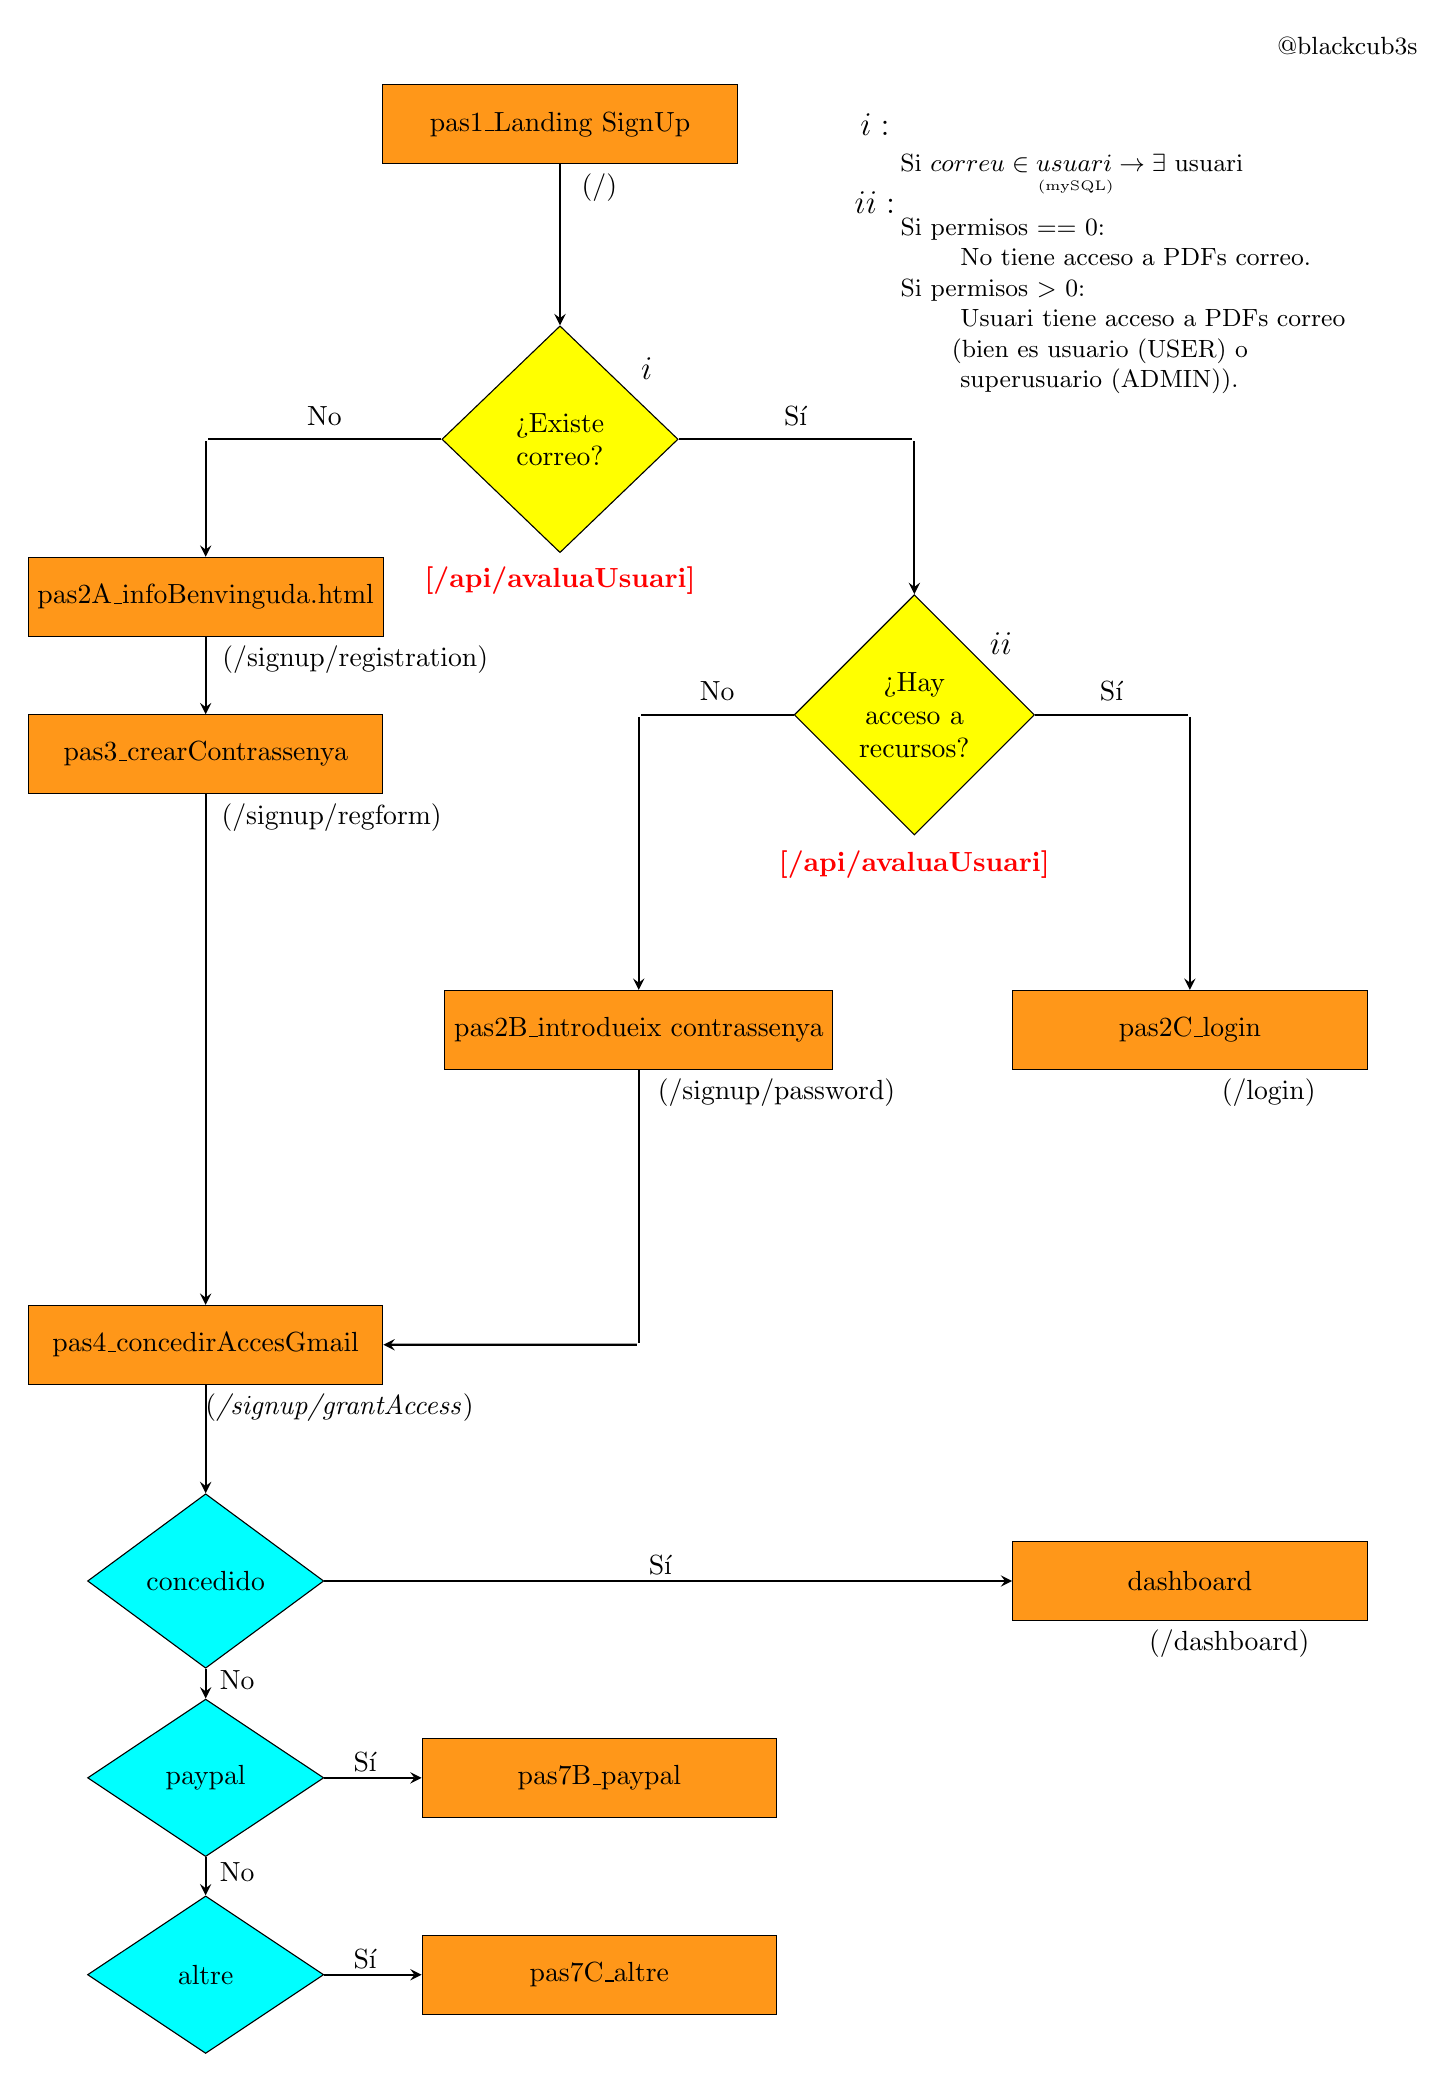
\begin{tikzpicture}[node distance=2cm]
	
	
	
	% Definici� de nodes
	
	
	\node (pas1) [trapeziSortida] {pas1\_Landing SignUp};
	\node (joMateix) [nomUsuari, right of=pas1, xshift=8cm, yshift=1cm] {@blackcub3s};
	\node (dec1) [decisionBackend, below of=pas1, yshift=-2cm,text width=1.75cm] {¿Existe\\correo?}; 
	\node (invisible1) [nodeNoDimensio, left of=dec1, xshift=-2.5cm] {};
	\node (pas2a) [trapeziSortida, below of=invisible1, xshift=0cm, yshift=0cm] {pas2A\_infoBenvinguda.html};
	\node (pas3) [trapeziSortida, below of=pas2a] {pas3\_crearContrassenya};
	
	\node (pas4) [trapeziSortida, below of=pas3, yshift=-5.5cm] {pas4\_concedirAccesGmail};
	
	\node (concedido) [decisionFrontend, below of=pas4, yshift=-1cm] {concedido};
	\node (paypal) [decisionFrontend, below of=concedido, yshift=-.5cm] {paypal};
	\node (altre) [decisionFrontend, below of=paypal, yshift=-.5cm] {altre};
	\node (dashboard) [trapeziSortida, right of=concedido, xshift=10.5cm] {dashboard};
	\node (pas7b) [trapeziSortida, right of=paypal, xshift=3cm] {pas7B\_paypal};
	\node (pas7c) [trapeziSortida, right of=altre, xshift=3cm] {pas7C\_altre};
	
	
	
	\node (invisible2) [nodeNoDimensio, right of=dec1, xshift=2.5cm] {};
	\node (dec2) [decisionBackend, below of=invisible2, yshift=-1.5cm, text width=1.5cm] {¿Hay acceso a recursos?};
	
	
	
	\node (invisible3) [nodeNoDimensio, left of=dec2, xshift=-1.5cm] {};
	\node (pas2b) [trapeziSortida, below of=invisible3, yshift=-2cm] {pas2B\_introdueix contrassenya};
	
	\node (invisible4) [nodeNoDimensio, right of=dec2, xshift=1.5cm] {};
	\node (pas2c) [trapeziSortida, below of=invisible4, yshift=-2cm] {pas2C\_login};
	
	\node (invisible5) [nodeNoDimensio, below of=pas2b,yshift=-2cm]{};
	
	
	%Nodes dummy (els del text de les url associats a cada trapezi de sortida)
	\node (dummy1) [below of=pas1, xshift=0.5cm, yshift=1.2cm] {(/)};  
	\node (dummy2) [below of=pas2a, xshift=1.9cm, yshift=1.2cm] {(/signup/registration)};  
	\node (dummy3) [below of=pas3, xshift=1.6cm, yshift=1.2cm] {(/signup/regform)};  
	
	\node (dummy5) [below of=pas4, xshift=1.7cm, yshift=1.2cm] {(\textit{/signup/grantAccess})};  
	 
	\node (dummy7) [below of=dashboard, xshift=.5cm, yshift=1.2cm] {(/dashboard)};  
	\node (dummy8) [below of=dec2, xshift=0cm, yshift=.1cm] {\textbf{\textcolor{red}{[/api/avaluaUsuari]}}};

	
\node (dummy9) [below of=dec1, xshift=0cm, yshift=.2cm] {\textbf{\textcolor{red}{[/api/avaluaUsuari]}}};

	\node (dummy10) [below of=pas2b, xshift=1.75cm, yshift=1.2cm] {(/signup/password)};  
	\node (dummy11) [below of=pas2c, xshift=1cm, yshift=1.2cm] {(/login)};  


	%nodes de comentari nota al "peu" (node de referEncia)
	\node (asterisc1sortida)[aspecteAsterisc, right of = dec1, yshift=.9cm, xshift=-.9cm]{$i$};
	\node (asterisc2sortida)[aspecteAsterisc, right of = dec2, yshift=.9cm, xshift=-.9cm]{$ii$};
	
	%nodes de comentari nota al "peu" (node referenciat -explicacio ampliada-)
	\node (asterisc1Arribada)[aspecteAsterisc, right of = pas1, yshift=0cm, xshift=2cm]{$i:$};
	\node (asterisc1Explicacio)[aspecteExplicacioAsterisc, right of = asterisc1Arribada, yshift=-.5cm, xshift=.5cm]{Si $correu \in usuari \rightarrow \exists $ usuari};
	\node (asterisc1ExplicacioComplement)[aspecteUltraPetit, below of = asterisc1Explicacio, yshift=1.7cm, xshift=.05cm]{(mySQL)};
	
	
	\node (asterisc2Arribada)[aspecteAsterisc, below of = asterisc1Arribada, yshift=1cm]{$ii:$};
	\node (asterisc2Explicacio)[aspecteExplicacioAsterisc, right of = asterisc2Arribada, yshift=-1.3cm, xshift=1.15cm] {
		\begin{tabular}{l}
			Si permisos == 0:\\
				\hspace{2em} No tiene acceso a PDFs correo.\\
			Si permisos $>$ 0:\\
				\hspace{2em} Usuari tiene acceso a PDFs correo\\\hspace{2em}(bien es usuario (USER) o \\\hspace{2em} superusuario (ADMIN)).			
		\end{tabular}
	};


	
	
	
	% Fletxes entre els nodes
	\draw [arrow] (pas1) -- (dec1);
	\draw [linia] (dec1) -- (invisible1) node[midway, yshift=0.3cm] {No};
	\draw [arrow] (invisible1) -- (pas2a);
	\draw [arrow] (pas2a) -- (pas3);
	\draw [arrow] (pas3) -- (pas4);


	\draw [arrow] (pas4) -- (concedido);
	
	\draw [arrow] (concedido) -- (paypal) node[midway, yshift=.05cm, xshift=.4cm] {No};
	\draw [arrow] (concedido) -- (dashboard)  node[midway, yshift=.2cm, xshift=-.1cm] {S\'{i}};
	\draw [arrow] (paypal) -- (altre) node[midway, yshift=.05cm, xshift=.4cm] {No};
	\draw [arrow] (paypal) -- (pas7b) node[midway, yshift=.2cm, xshift=-.1cm] {S\'{i}};
	\draw [arrow] (altre) -- (pas7c)  node[midway, yshift=.2cm, xshift=-.1cm] {S\'{i}};
	

	\draw [linia] (dec1) --  (invisible2) node[midway, yshift=0.3cm] {S\'{i}};
	\draw [arrow] (invisible2) --  (dec2);
	
	\draw [linia] (dec2) -- (invisible3) node[midway, yshift=0.3cm] {No};
	\draw [arrow] (invisible3) -- (pas2b);
	
	\draw [linia] (dec2) -- (invisible4) node[midway, yshift=0.3cm] {S\'{i}};
	\draw [arrow] (invisible4) -- (pas2c);
	
	\draw [linia] (pas2b) -- (invisible5) node[midway, yshift=0.3cm] {};
	\draw [arrow] (invisible5) -- (pas4);
	
	
	\end{tikzpicture}
	
\end{document}
